\subsection{Lineare Gleichungen mit Parametern}
\begin{LA}
    {Einführung}{}
    \begin{center}
        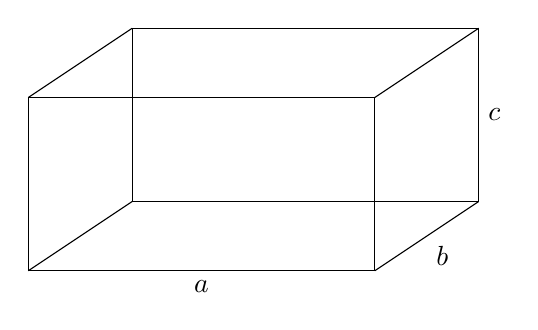
\begin{tikzpicture}[scale=1.1]
            % Vorderseite
            \coordinate (A) at (0,0);
            \coordinate (B) at (4,0);
            \coordinate (C) at (4,2);
            \coordinate (D) at (0,2);

            % Rückseite
            \coordinate (E) at (1.2,0.8);
            \coordinate (F) at (5.2,0.8);
            \coordinate (G) at (5.2,2.8);
            \coordinate (H) at (1.2,2.8);

            % Vorderseite
            \draw (A) -- node[midway,below] {\(a\)} (B)
            -- (C)
            -- (D)
            -- cycle;

            % Verbindung zur Rückseite
            \draw (A) -- (E);
            \draw (B) -- node[midway,below right] {\(b\)} (F);
            \draw (C) -- (G);
            \draw (D) -- (H);

            % Rückseite
            \draw (E) -- (F)
            -- node[midway,right] {\(c\)} (G)
            -- (H)
            -- cycle;
        \end{tikzpicture}
    \end{center}

    Die Oberfläche eines Quaders mit den Kanten \(a\), \(b\) und \(c\) kann man mit folgender Formel berechnen:
    \[
        A = 2(ab+ac+bc)
    \]

    \begin{enumerate}
        \item Berechnen Sie die Länge der Kante \(c\), falls
              \begin{enumerate}
                  \item \(A=76\,\mathrm{m}^2,\quad a=2\,\mathrm{m},\quad b=4\,\mathrm{m}\)
                  \item \(A=62\,\mathrm{m}^2,\quad a=3\,\mathrm{m},\quad b=7\,\mathrm{m}\)
                  \item \(A=38\,\mathrm{m}^2,\quad a=1\,\mathrm{m},\quad b=4\,\mathrm{m}\)
                  \item \(A=96\,\mathrm{m}^2,\quad a=4\,\mathrm{m},\quad b=4\,\mathrm{m}\)
              \end{enumerate}

        \item Geben Sie eine Formel an, mit der man die Länge der Kante \(c\) direkt aus der Fläche \(A\) und den Kanten \(a\) und \(b\) berechnen kann. Überprüfen Sie anschliessend die Resultate aus Aufgabe 1) mit der gefundenen Formel.
    \end{enumerate}
\end{LA}





\clearpage
Wir haben Parameter bereits einmal verwendet, als wir den Satz von Vieta besprochen haben. Damals haben wir Terme der Form
\[
    (x+2)(x+6)
\]
oder
\[
    (x+1)(x+3)
\]
ausmultipliziert. Damit wir diese Multiplikationen nicht jedes Mal von vorne ausführen mussten, haben wir die Parameter \(a\) und \(b\) eingeführt und eine Formel aufgestellt:
\[
    (x+a)(x+b)=x^2+(a+b)x+ab.
\]

Parameter dienen dazu, viele ähnliche Probleme auf einmal zu lösen. Genauso war es in der Einführungsaufgabe. In der ersten Aufgabe ist immer dasselbe gesucht: die Länge von \(c\). Es ändern sich nur die Werte von \(A\), \(a\) und \(b\). Man kann nun diese Aufgaben unabhängig voneinander lösen. Dazu muss man jedes Mal eine Gleichung lösen. Oder man löst die Gleichung nur einmal in allgemeiner Form auf:
\[
    A=2(ab+ac+bc).
\]

Da wir die Länge von \(c\) bestimmen möchten, ist \(c\) die Unbekannte und \(A\), \(a\) und \(b\) die Parameter.

\[
    \begin{aligned}
        A     & = 2(ab+ac+bc) &  & \mid \text{TU} \\
        A     & = 2ab+2ac+2bc &  & \mid -2ab      \\
        A-2ab & = 2ac+2bc
    \end{aligned}
\]

Nun ist die Unbekannte \(c\) rechts und alles andere links vom Gleichheitszeichen. Um zu verstehen, wie es nun weitergeht, überlegen wir uns kurz, wie diese Situation aussehen würde, wenn \(A\), \(a\) und \(b\) ganz konkrete Zahlen wären. Für \(A=76\), \(a=2\) und \(b=4\) zum Beispiel erhalten wir:
\[
    76-2\cdot2\cdot4=2\cdot2c+2\cdot4c.
\]

In diesem konkreten Fall stünde auf der rechten Seite insgesamt \(12c\) und wir würden die Gleichung durch \(12\) teilen, um das Resultat zu erhalten.

Jetzt blicken wir wieder auf unsere allgemeine Gleichung
\[
    A-2ab=2ac+2bc.
\]

Wie viel mal \(c\) steht eigentlich auf der rechten Seite? Das erkennt man, wenn man \(c\) \textbf{ausklammert}:
\[
    A-2ab=(2a+2b)c.
\]

Auf der rechten Seite kommt die Grösse \(c\) insgesamt \((2a+2b)\)-mal vor. Dividiert man nun die Gleichung durch \((2a+2b)\), erhält man die gesuchte Formel für \(c\):
\[
    c=\frac{A-2ab}{2a+2b}.
\]

\begin{satz}{Rezept zum Lösen von linearen Gleichungen mit Parametern}{}
    \begin{enumerate}
        \item Mit Termumformungen beide Seiten vereinfachen.
        \item Mit Äquivalenzumformungen die Unbekannte auf die eine Seite und alles andere auf die andere Seite bringen.
        \item \textbf{Die Unbekannte ausklammern.}
        \item Die Gleichung durch den Vorfaktor der Unbekannten teilen.
    \end{enumerate}
\end{satz}
\begin{bsp}{Lineare Gleichung mit Parametern}{}
    Gesucht ist \(x\):
    \[
        4-2(ax+b)=b(x-1)
    \]
    \vspace*{4cm}
\end{bsp}

In der Physik, in der Geometrie und in vielen anderen Anwendungsgebieten werden Grössen durch eine Gleichung in Verbindung gebracht. Je nachdem, welche dieser Grössen gesucht oder gegeben sind, muss man die Gleichung nach der einen oder anderen Variable auflösen.

\begin{bsp}{Flächeninhalt eines Trapezes}{}
    Die Fläche \(A\) eines Trapezes, dessen beiden Grundseiten \(a\) und \(c\) und dessen Höhe \(h\) sind, wird durch die Formel
    \[
        A=\frac{a+c}{2}\cdot h
    \]
    beschrieben.

    Diese Gleichung ist praktisch, wenn \(a\), \(c\) und \(h\) gegeben sind und \(A\) gesucht wird. Wenn hingegen \(h\) gesucht ist, sollte man die Gleichung nach \(h\) auflösen:
    \[
        A=\frac{a+c}{2}\cdot h
    \]

    \clearpage

    Wenn jedoch \(a\) gesucht wird, sollte man sie entsprechend nach \(a\) auflösen:
    \[
        A=\frac{a+c}{2}\cdot h
    \]

    \vspace{3cm}
\end{bsp}

\begin{ueb}
    {Lineare Gleichung mit Parametern}{}
    \begin{enumerate}
        \item Lösen Sie die Gleichung nach \(x\) auf. Bewahren Sie die Lösungen sicher auf, Sie werden sie in einer späteren Aufgabe wieder benötigen.

              \begin{enumerate}
                  \item \(cx+c=dx\)
                  \item \(ax=a^2+a\)
                  \item \(qx=1-px\)
                  \item \(qx=-px\)
                  \item \(ax-b=2b+x\)
                  \item \((a+b)x=a^2+2ab+b^2\)
                  \item \(x-p=p^2-px\)
                  \item \(q+3qx=x\)
              \end{enumerate}
    \end{enumerate}
\end{ueb}
\clearpage
\emph{Lösungen:}
\begin{enumerate}
    \item \(x=\dfrac{c}{d-c}\)
    \item \(x=a+1\)
    \item \(x=\dfrac{1}{p+q}\)
    \item \(x=0\)
    \item \(x=\dfrac{3b}{a-1}\)
    \item \(x=a+b\)
    \item \(x=p\)
    \item \(x=\dfrac{q}{1-3q}\)
\end{enumerate}









